\begin{figure}[H]
    \centering
    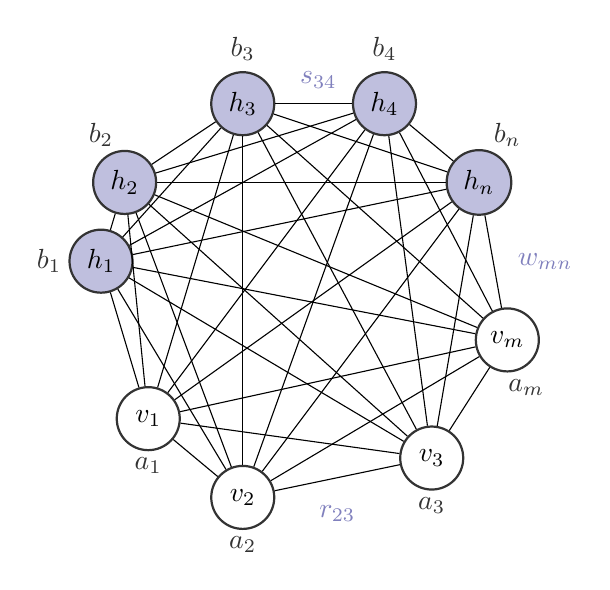
\begin{tikzpicture}
    \tikzset{cir/.style={circle,draw=black!80,thick,minimum size=0.8cm},y=0.6cm,font=\sffamily}
    \definecolor{bluebell}{rgb}{0.5, 0.5, 0.74}
    \tikzset{cirblue/.style={circle,draw=black!80,thick,
        fill=bluebell!50,minimum size=0.8cm},y=0.6cm,font=\sffamily}


    
    \begin{scope}[rotate=90]
    \node[cir] (b1) at (-2,0) {$v_1$};
    \node[cir] (b2) at (-3,-1*2) {$v_2$};
    \node[cir] (b3) at (-2.5,-3*2) {$v_3$};
    \node[cir] (b4) at (-1,-3.8*2) {$v_m$};
    \node[cirblue] (c1) at (0,1) {$h_1$};
    \node[cirblue] (c2) at (1,-1*0.5+1) {$h_2$};
    \node[cirblue] (c3) at (2,-1.5*2+1) {$h_3$};
    \node[cirblue] (c4) at (2,-3*2+1) {$h_4$};
    \node[cirblue] (c5) at (1,-3*2-1) {$h_n$};
    
    \draw (-2.6, 0) node[black!80] {$a_1$};
    \draw (-3.6, -1*2) node[black!80] {$a_2$};
    \draw (-3.1, -2*3) node[black!80] {$a_3$};
    \draw (-1.6, -4*2) node[black!80] {$a_m$};
    \draw (0, 2.1) node[black!80] {$b_1$};
    \draw (1.6, 1) node[black!80] {$b_2$};
    \draw (2.7,-1.5*2+1) node[black!80] {$b_3$};
    \draw (2.7, -3*2+1) node[black!80] {$b_4$};
    \draw (1.6,-3*2.2-1) node[black!80] {$b_n$};
    \draw (0, -4*2.1) node[bluebell!100] {$w_{mn}$};
    \draw (2.3,-2.3*2+1) node[bluebell!100] {$s_{34}$};
    \draw (-3.2,-2.5*2+1) node[bluebell!100] {$r_{23}$};
    
    
    \foreach \cnto [count=\i] in {b1,b2,b3,b4,c1,c2,c3,c4,c5} {
        \foreach \cntt [count=\j] in {b1,b2,b3,b4,c1,c2,c3,c4,c5} {
            \ifnum \i<\j
                \draw (\cnto) -- (\cntt);
            \fi
        }
    }
    
    \end{scope}
    \end{tikzpicture}
    \caption{Schematics of a BM. The nodes coloured in light purple represent the hidden layer of the network. Letters $s$ and $r$ represent the intra-layer connection, while and $w$ represents outer-layer connections.}
    \label{fig:bm}
\end{figure}




